\chapter{MÔ HÌNH SINH HỌC--KINH TẾ VÀ PHÂN TÍCH ỔN ĐỊNH}
\label{ch:bioeconomic}

\textit{(Nội dung chi tiết của chương này sẽ được phát triển đầy đủ trong giai đoạn tiếp theo):}

\section{Mô hình sinh học--kinh tế mở rộng}
\label{sec:ecological_economic}

Bên cạnh mối quan hệ con mồi--vật săn mồi giữa cá Atlantic Menhaden và cá Striped Bass, hoạt động khai thác của con người cũng là một yếu tố quan trọng ảnh hưởng đến động lực quần thể của hai loài. Cả hai loài không chỉ giữ vai trò quan trọng trong hệ sinh thái vịnh Chesapeake mà còn mang lại giá trị kinh tế đáng kể thông qua hoạt động đánh bắt thủy sản.

Do đó, một vấn đề đặt ra là xác định mức độ khai thác phù hợp sao cho có thể đạt được lợi ích kinh tế nhưng vẫn duy trì sự ổn định và bền vững của quần thể hai loài trong dài hạn. Để nghiên cứu vấn đề này, mô hình Lotka--Volterra tổng quát được mở rộng bằng cách bổ sung tác động của hoạt động khai thác và một hàm lợi nhuận kinh tế.

\subsection{Mô hình sinh học--kinh tế}
\label{subsec:bionomic_model}

Giả sử cả cá Atlantic Menhaden và cá Striped Bass đều được khai thác theo giả thiết \textit{catch per unit effort}, tức lượng cá đánh bắt được tỷ lệ thuận với cường độ khai thác và kích thước quần thể hiện tại.

Ký hiệu
\begin{itemize}
    \item $x(t)$ là kích thước quần thể Atlantic Menhaden tại thời điểm $t$;
    \item $y(t)$ là kích thước quần thể Striped Bass tại thời điểm $t$;
    \item $E_1$, $E_2$ là cường độ khai thác của hai loài;
    \item $q_1$, $q_2$ là hệ số khả năng đánh bắt (\textit{catchability coefficient})  của hai loài.
\end{itemize}

Khi đó, $q_1E_1x$ và $q_2E_2y$ lần lượt biểu diễn lượng Atlantic Menhaden và Striped Bass bị khai thác trên một đơn vị thời gian.

\vspace{0.3cm}

Bên cạnh tác động đến quần thể, hoạt động khai thác còn được xét dưới góc độ kinh tế. Ký hiệu:
\begin{itemize}
    \item $p_1$, $p_2$ là giá bán trên một đơn vị sinh khối của Atlantic Menhaden và Striped Bass;
    \item $c_1$, $c_2$ là chi phí trên một đơn vị cường độ khai thác của hai loài.
\end{itemize}

Do lượng khai thác của hai loài lần lượt là $q_1E_1x$ và $q_2E_2y$, doanh thu tương ứng là $p_1q_1E_1x$ và $p_2q_2E_2y$, trong khi chi phí khai thác là $c_1E_1$ và $c_2E_2$. Vì vậy, tổng lợi nhuận từ hoạt động khai thác hai loài được xác định bởi
\[
\pi(E_1,E_2)
=
(p_1q_1x-c_1)E_1
+
(p_2q_2y-c_2)E_2.
\]

Kết hợp mô hình động lực quần thể với hoạt động khai thác và hàm lợi nhuận, ta thu được mô hình sinh học--kinh tế:
\begin{equation}
\begin{cases}
\dfrac{dx}{dt}
=
x(r-ax-by)-q_1E_1x, \\[8pt]

\dfrac{dy}{dt}
=
y(-e-cy+dx)-q_2E_2y, \\[8pt]

\pi(E_1,E_2)
=
(p_1q_1x-c_1)E_1
+
(p_2q_2y-c_2)E_2,
\end{cases}
\label{eq:bionomic_model}
\end{equation}
với điều kiện ban đầu
\[
x(0)\geq 0,
\qquad
y(0)\geq 0.
\]

\subsection{Tính chất của nghiệm}
\label{subsec:positivity_boundedness}

\subsubsection{Tính không âm}

Từ phương trình thứ nhất của mô hình \eqref{eq:bionomic_model}, ta có
\[
\frac{1}{x}\frac{dx}{dt}
=
r-ax-by-q_1E_1.
\]

Đặt
\[
\phi_1(x,y)
=
r-ax-by-q_1E_1.
\]

Khi đó
\[
\frac{dx}{x}
=
\phi_1(x,y)\,dt.
\]

Lấy tích phân trên khoảng $[0,t]$, ta được
\begin{equation}
x(t)
=
x(0)
\exp
\left(
\int_0^t
\phi_1(x(s),y(s))\,ds
\right).
\label{eq:x_positive}
\end{equation}

Do
\[
x(0)\geq 0
\]
và hàm mũ luôn dương, suy ra
\[
x(t)\geq 0,
\qquad \forall t\geq 0.
\]

Tương tự, từ phương trình thứ hai,
\[
\frac{1}{y}\frac{dy}{dt}
=
-e-cy+dx-q_2E_2.
\]

Đặt
\[
\phi_2(x,y)
=
-e-cy+dx-q_2E_2.
\]

Ta thu được
\begin{equation}
y(t)
=
y(0)
\exp
\left(
\int_0^t
\phi_2(x(s),y(s))\,ds
\right).
\label{eq:y_positive}
\end{equation}

Vì $y(0)\geq 0$, suy ra
\[
y(t)\geq 0,
\qquad \forall t\geq 0.
\]

Như vậy, nếu điều kiện ban đầu không âm thì quần thể của cả hai loài luôn không âm trong suốt quá trình phát triển của hệ.

\subsubsection{Tính bị chặn}

Trước hết, xét phương trình của Atlantic Menhaden. Vì các tham số và $x,y$ đều không âm nên
\[
\frac{dx}{dt}
=
x(r-ax-by)-q_1E_1x
\leq
x(r-ax).
\]

Xét phương trình logistic
\begin{equation}
\frac{dx}{dt}=x(r-ax).
\label{eq:logistic}
\end{equation}

Tách biến và phân tích thành phân số đơn:
\begin{equation}
\frac{dx}{x(r-ax)}
=
dt
\quad\Longleftrightarrow\quad
\left(
\frac{1}{rx}
+
\frac{a}{r(r-ax)}
\right)dx
=
dt.
\end{equation}

Lấy tích phân hai vế:
\begin{align}
\int
\left(
\frac{1}{rx}
+
\frac{a}{r(r-ax)}
\right)dx
&=
\int dt
\nonumber\\
\frac{1}{r}\ln x
-
\frac{1}{r}\ln(r-ax)
&=
t+C_1
\nonumber\\
\ln\left(\frac{x}{r-ax}\right)
&=
rt+C_2.
\end{align}

Lấy hàm mũ hai vế và đặt $C=e^{C_2}>0$, ta được
\[
\frac{x}{r-ax}=Ce^{rt}.
\]

Từ đó,
\[
x
=
Ce^{rt}(r-ax)
\quad\Longrightarrow\quad
x(1+aCe^{rt})
=
Cr e^{rt},
\]
suy ra
\begin{equation}
x(t)
=
\frac{Cr e^{rt}}{1+aCe^{rt}}
=
\frac{Cr}{aC+e^{-rt}}.
\label{eq:logistic_solution}
\end{equation}

Khi $t\to\infty$ thì
\[
x(t)\longrightarrow \frac{Cr}{aC}=\frac{r}{a},
\]
suy ra $x(t)$ bị chặn.

\vspace{0.3cm}

Để chứng minh $y(t)$ bị chặn, xét phương trình thứ hai của hệ:
\begin{equation}
\frac{dy}{dt}
=
y(-e-cy+dx)-q_2E_2y
=
-ey-cy^2+dxy-q_2E_2y.
\label{eq:y_equation}
\end{equation}

Từ phương trình thứ nhất,
\[
\frac{dx}{dt}
=
x(r-ax)-bxy-q_1E_1x,
\]
suy ra
\begin{equation}
xy
=
\frac{1}{b}
\left(
x(r-ax)-q_1E_1x-\frac{dx}{dt}
\right).
\label{eq:xy_expression}
\end{equation}

Thế \eqref{eq:xy_expression} vào \eqref{eq:y_equation}, ta được
\begin{equation}
\frac{dy}{dt}
=
-ey-cy^2
+
\frac{d}{b}
\left(
x(r-ax)-q_1E_1x-\frac{dx}{dt}
\right)
-q_2E_2y.
\end{equation}

Đặt $\gamma=\dfrac{d}{b}$, khi đó
\[
\frac{dy}{dt}
+
\gamma\frac{dx}{dt}
=
\gamma x(r-ax)
-
\gamma q_1E_1x
-
ey-cy^2-q_2E_2y.
\]

Chia hai vế cho $\gamma$:
\[
\frac{dx}{dt}
+
\frac{1}{\gamma}\frac{dy}{dt}
=
x(r-ax)
-
q_1E_1x
-
\frac{1}{\gamma}
\left(
ey+cy^2+q_2E_2y
\right).
\]

Đặt $w(t)=x(t)+\dfrac{y(t)}{\gamma}$, suy ra
\begin{equation}
\frac{dw}{dt}
=
x(r-ax)
-
q_1E_1x
-
\frac{1}{\gamma}
\left(
ey+cy^2+q_2E_2y
\right).
\label{eq:w_derivative}
\end{equation}

Vì $cy^2\geq 0$, từ \eqref{eq:w_derivative} suy ra
\[
\frac{dw}{dt}
\leq
x(r-ax)-q_1E_1x
-\frac{y}{\gamma}(e+q_2E_2).
\]

Mặt khác, hàm $f(x)=x(r-ax)$ đạt giá trị lớn nhất tại
$x=\dfrac{r}{2a}$, với
\[
f_{\max}=\frac{r^2}{4a}.
\]

Đặt $\delta=\min\{q_1E_1,q_2E_2,e\}$, khi đó
$q_1E_1\geq\delta$ và $e+q_2E_2\geq\delta$. Do đó,
\begin{align}
\frac{dw}{dt}
&\leq
\frac{r^2}{4a}
-\delta x
-\delta\frac{y}{\gamma}
\nonumber\\
&=
\frac{r^2}{4a}
-\delta w.
\end{align}

Suy ra
\begin{equation}
\frac{dw}{dt}+\delta w
\leq
\frac{r^2}{4a}.
\label{eq:w_inequality}
\end{equation}

Nhân hai vế của \eqref{eq:w_inequality} với $e^{\delta t}$:
\[
e^{\delta t}\frac{dw}{dt}
+
\delta e^{\delta t}w
\leq
\frac{r^2}{4a}e^{\delta t}.
\]

Vì
\[
\frac{d}{dt}\left(e^{\delta t}w(t)\right)
=
e^{\delta t}\frac{dw}{dt}
+
\delta e^{\delta t}w,
\]
nên
\[
\frac{d}{dt}\left(e^{\delta t}w(t)\right)
\leq
\frac{r^2}{4a}e^{\delta t}.
\]

Lấy tích phân từ $0$ đến $t$, ta được
\[
e^{\delta t}w(t)-w(0)
\leq
\frac{r^2}{4a\delta}
\left(e^{\delta t}-1\right),
\]
hay
\begin{equation}
w(t)
\leq
e^{-\delta t}
\left(
w(0)-\frac{r^2}{4a\delta}
\right)
+
\frac{r^2}{4a\delta}.
\label{eq:w_bound}
\end{equation}

Khi $t\to\infty$ thì
\[
w(t)\leq \frac{r^2}{4a\delta},
\]
suy ra $w(t)$ bị chặn. Vì
$w(t)=x(t)+\dfrac{y(t)}{\gamma}$ và $x(t),y(t)\geq0$, ta có
\[
0\leq \frac{y(t)}{\gamma}\leq w(t),
\]
do đó $y(t)$ cũng bị chặn.

\vspace{0.3cm}

Từ các kết quả trên, miền nghiệm có dạng
\begin{equation}
\Omega
=
\left\{
(x,y)\ \middle|\
0\leq x\leq \frac{r}{a},
\quad
0\leq x+\frac{y}{\gamma}\leq L
\right\},
\qquad
\gamma=\frac{d}{b},
\qquad
L=\frac{r^2}{4a\delta}.
\label{eq:omega}
\end{equation}

\begin{figure}[htbp]
    \centering
    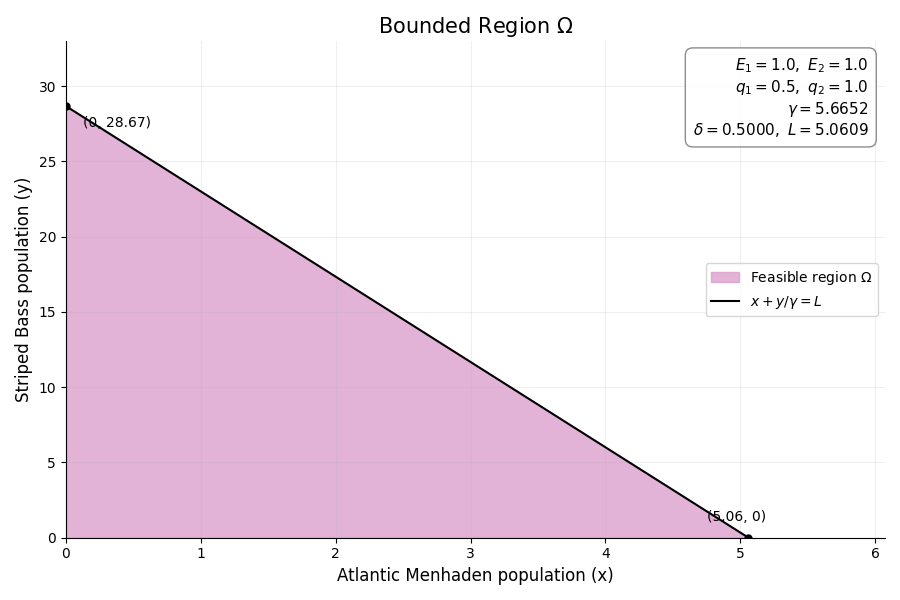
\includegraphics[width=0.85\textwidth]{images/region_omega.png}
    \caption{Minh họa miền giới hạn $\Omega$ của hệ với
    bộ tham số trong Bảng 1.}
    \label{fig:region_omega}
\end{figure}

\subsection{Xác định các điểm cân bằng của mô hình}
\label{subsec:bionomic_equilibrium}

Cân bằng sinh học--kinh tế đạt được khi quần thể của hai loài không còn thay đổi theo thời gian và tổng doanh thu từ hoạt động khai thác bằng tổng chi phí khai thác. Do đó, tại trạng thái cân bằng ta có
\[
\frac{dx}{dt}=0,
\qquad
\frac{dy}{dt}=0,
\qquad
\pi(E_1,E_2)=0.
\]

Giả sử điểm cân bằng sinh học--kinh tế có dạng
\[
P(x_B,y_B,E_{1B},E_{2B}),
\]
trong đó $x_B,y_B$ là kích thước quần thể của cá Atlantic Menhaden và Striped Bass; $E_{1B},E_{2B}$ là cường độ khai thác tương ứng tại trạng thái cân bằng.

\vspace{0.3cm}

Khi đó, điểm cân $P$ phải thỏa mãn hệ
\begin{equation}
\begin{cases}
r-ax-by-q_1E_1=0,\\[4pt]
-e-cy+dx-q_2E_2=0,\\[4pt]
(p_1q_1x-c_1)E_1+(p_2q_2y-c_2)E_2=0.
\end{cases}
\label{eq:bionomic_equilibrium_system}
\end{equation}

\subsubsection{Trường hợp 1: Chỉ khai thác cá Striped Bass (Vật săn mồi)}

Xét trường hợp $E_1=0$ và $E_2\neq 0$, tức hoàn toàn không khai thác cá Atlantic Menhaden (con mồi) .
Khi đó, phương trình lợi nhuận trong hệ
\eqref{eq:bionomic_equilibrium_system} trở thành
\[
(p_2q_2y-c_2)E_2=0.
\]

Vì $E_2\neq 0$, suy ra
\[
p_2q_2y-c_2=0
\quad\Longleftrightarrow\quad
y_B=\frac{c_2}{p_2q_2}.
\]

Thế $y_B$ vào phương trình thứ nhất của hệ \eqref{eq:bionomic_equilibrium_system}, ta được
\[
r-ax_B-by_B=0
\quad\Longleftrightarrow\quad
x_B=\frac{r}{a}-\frac{bc_2}{ap_2q_2}.
\]

Tiếp tục thế $x_B$ và $y_B$ vào phương trình thứ hai của hệ \eqref{eq:bionomic_equilibrium_system}, ta được:
\[
-e-cy_B+dx_B-q_2E_{2B}=0
\quad\Longleftrightarrow\quad
E_{2B}
=
-\frac{e}{q_2}
-
\frac{cc_2}{p_2q_2^2}
+
\frac{d}{q_2}
\left(
\frac{r}{a}
-
\frac{bc_2}{ap_2q_2}
\right).
\]

Do đó, điểm cân bằng sinh học--kinh tế trong trường hợp chỉ khai thác
Striped Bass là
\[
P_1
=
\left(
\frac{r}{a}-\frac{bc_2}{ap_2q_2},
\frac{c_2}{p_2q_2},
0,
E_{2B}
\right).
\]

Điểm cân bằng này tồn tại khi $x_B>0$ và $E_{2B}>0$, tương đương với:
\[
\frac{r}{a}>\frac{bc_2}{ap_2q_2},
\qquad
\frac{d}{q_2}
\left(
\frac{r}{a}-\frac{bc_2}{ap_2q_2}
\right)
>
\frac{e}{q_2}
+
\frac{cc_2}{p_2q_2^2}.
\]

\subsubsection{Trường hợp 2: Chỉ khai thác cá Atlantic Menhaden (con mồi)}

Xét trường hợp $E_1\neq 0$ và $E_2=0$, tức không khai thác cá Striped Bass (Vật săn mồi).
Khi đó, phương trình lợi nhuận trong hệ
\eqref{eq:bionomic_equilibrium_system} trở thành
\[
(p_1q_1x-c_1)E_1=0.
\]

Vì $E_1\neq 0$, suy ra
\[
p_1q_1x-c_1=0
\quad\Longleftrightarrow\quad
x_B=\frac{c_1}{p_1q_1}.
\]

Thế $x_B$ vào phương trình thứ hai của hệ
\eqref{eq:bionomic_equilibrium_system}, ta được
\[
-e-cy_B+dx_B=0
\quad\Longleftrightarrow\quad
y_B=
\frac{dc_1}{cp_1q_1}-\frac{e}{c}.
\]

Tiếp tục thế $x_B$ và $y_B$ vào phương trình thứ nhất của hệ
\eqref{eq:bionomic_equilibrium_system}, ta được
\[
r-ax_B-by_B-q_1E_{1B}=0
\quad\Longleftrightarrow\quad
E_{1B}
=
\frac{r}{q_1}
-
\frac{ac_1}{p_1q_1^2}
-
\frac{b}{q_1}
\left(
\frac{dc_1}{cp_1q_1}-\frac{e}{c}
\right).
\]

Do đó, điểm cân bằng sinh học--kinh tế trong trường hợp chỉ khai thác
Atlantic Menhaden là
\[
P_2
=
\left(
\frac{c_1}{p_1q_1},
\frac{dc_1}{cp_1q_1}-\frac{e}{c},
E_{1B},
0
\right).
\]

Điểm cân bằng này tồn tại khi $y_B>0$ và $E_{1B}>0$, tương đương với:
\[
\frac{dc_1}{cp_1q_1}>\frac{e}{c},
\qquad
\frac{r}{q_1}
-
\frac{ac_1}{p_1q_1^2}
>
\frac{b}{q_1}
\left(
\frac{dc_1}{cp_1q_1}-\frac{e}{c}
\right).
\]

\subsubsection{Trường hợp 3: Không khai thác cả hai loài}

Xét trường hợp $E_1=0$ và $E_2=0$, tức không khai thác cả Atlantic Menhaden (con mồi) và Striped Bass (vật săn mồi).

Khi đó, hệ \eqref{eq:bionomic_equilibrium_system} trở thành
\[
\begin{cases}
r-ax-by=0,\\
-e-cy+dx=0.
\end{cases}
\]

Đây là hệ phương trình bậc nhất hai ẩn $x$ và $y$. Giải hệ, ta thu được
\[
x^*
=
\frac{rc+be}{ac+bd},
\qquad
y^*
=
\frac{rd-ae}{ac+bd}.
\]

Do đó, điểm cân bằng sinh học trong trường hợp không khai thác cả hai loài là
\[
P_3
=
\left(
\frac{rc+be}{ac+bd},
\frac{rd-ae}{ac+bd},
0,
0
\right).
\]

Để điểm cân bằng có ý nghĩa sinh học, cần $x^*>0$ và $y^*>0$. 

Dễ dàng nhận thấy $x^*>0$ do các tham số đều dương. 

Mặt khác,
$y^*>0 \Longrightarrow rd>ae$.

Vì vậy, điểm cân bằng $P_3$ tồn tại nếu:
\[
rd>ae.
\]

\subsubsection{Trường hợp 4: Khai thác đồng thời cả hai loài}

Xét trường hợp $E_1\neq 0$ và $E_2\neq 0$, tức đồng thời khai thác cả Atlantic Menhaden (con mồi) và Striped Bass (vật săn mồi).

Giả sử chi phí khai thác không vượt quá doanh thu tương ứng
của mỗi loài, tức là
\[
    c_1 \leq p_1q_1x,\qquad c_2 \leq p_2q_2y.
\]
Khi đó, lợi nhuận từ mỗi hoạt động khai thác đều không âm:
\[
    p_1q_1x-c_1 \geq 0,\qquad p_2q_2y-c_2 \geq 0.
\]
Mặt khác, do $E_1>0$, $E_2>0$ và tổng lợi nhuận
tại trạng thái cân bằng sinh học--kinh tế bằng $0$, ta có
\[
    (p_1q_1x-c_1)E_1+(p_2q_2y-c_2)E_2=0.
\]
Vì tổng của hai số không âm bằng $0$ nên từng số
phải bằng $0$. Do đó,
\[
    \begin{cases}
        p_1q_1x-c_1=0,\\
        p_2q_2y-c_2=0
    \end{cases}
    \Longleftrightarrow
    \begin{cases}
        x_B=\dfrac{c_1}{p_1q_1},\\[6pt]
        y_B=\dfrac{c_2}{p_2q_2}.
    \end{cases}
\]

Khi đó, để phương trình lợi nhuận trong hệ
\eqref{eq:bionomic_equilibrium_system} bằng $0$, ta cần:
\[
p_1q_1x_B-c_1=0,
\qquad
p_2q_2y_B-c_2=0,
\]
suy ra
\[
x_B=\frac{c_1}{p_1q_1},
\qquad
y_B=\frac{c_2}{p_2q_2}.
\]

Thế $x_B$ và $y_B$ vào phương trình thứ nhất của hệ
\eqref{eq:bionomic_equilibrium_system}, ta được
\[
r-ax_B-by_B-q_1E_{1B}=0
\quad\Longleftrightarrow\quad
E_{1B}
=
\frac{r}{q_1}
-
\frac{ac_1}{p_1q_1^2}
-
\frac{bc_2}{p_2q_1q_2}.
\]

Tương tự, thế $x_B$ và $y_B$ vào phương trình thứ hai:
\[
-e-cy_B+dx_B-q_2E_{2B}=0
\quad\Longleftrightarrow\quad
E_{2B}
=
-\frac{e}{q_2}
-
\frac{cc_2}{p_2q_2^2}
+
\frac{dc_1}{p_1q_1q_2}.
\]

Do đó, điểm cân bằng sinh học--kinh tế trong trường hợp khai thác đồng thời cả hai loài là
\[
P_4
=
\left(
\frac{c_1}{p_1q_1},
\frac{c_2}{p_2q_2},
E_{1B},
E_{2B}
\right).
\]

Vì $x_B>0$ và $y_B>0$ khi các tham số đều dương, điểm cân bằng $P_4$ tồn tại khi
$E_{1B}>0$ và $E_{2B}>0$, tương đương với
\[
\frac{r}{q_1}
>
\frac{ac_1}{p_1q_1^2}
+
\frac{bc_2}{p_2q_1q_2},
\qquad
\frac{dc_1}{p_1q_1q_2}
>
\frac{e}{q_2}
+
\frac{cc_2}{p_2q_2^2}.
\]


\subsection{Phân tích tính ổn định và khả năng phục hồi của hệ sinh thái}

Để kiểm tra tính ổn định của hệ khi có hoạt động khai thác,
ta xét ma trận Jacobian:
\begin{equation}
    J(x,y)=
    \begin{pmatrix}
        r-2ax-by-q_1E_1 & -bx\\
        dy & -e-2cy+dx-q_2E_2
    \end{pmatrix}.
\end{equation}


Với ma trận Jacobian cấp hai, các trị riêng
là nghiệm của phương trình đặc trưng
\[
    \lambda^2-\operatorname{tr}(J)\lambda
    +\det(J)=0.
\]
Theo tiêu chuẩn Routh--Hurwitz, nếu
$\operatorname{tr}(J)<0$ và $\det(J)>0$
thì các trị riêng đều có phần thực âm,
suy ra điểm cân bằng ổn định tiệm cận.

Bên cạnh đó, để đánh giá khả năng
phục hồi sau nhiễu động nhỏ, xét thời gian hồi phục
đặc trưng $\tau$ và khả năng phục hồi $R$:
\begin{equation}
    \tau=-\frac{1}{\operatorname{Re}(\lambda_m)},
    \qquad R=\frac{1}{\tau},
\end{equation}
trong đó $\lambda_m$ là trị riêng có phần thực lớn nhất
của ma trận Jacobian tại điểm cân bằng ổn định.

\subsubsection{Trường hợp 1: Chỉ khai thác cá Striped Bass (Vật săn mồi)}

Xét trường hợp $E_1=0$, $E_2>0$. Tại điểm cân bằng
cùng tồn tại $(\hat{x},\hat{y})$, ta có
\[
    \begin{cases}
        a\hat{x}+b\hat{y}=r,\\
        d\hat{x}-c\hat{y}=e+q_2E_2.
    \end{cases}
\]

Giải hệ, ta thu được
\[
    \hat{x}=\frac{b(e+q_2E_2)+rc}{ac+bd},
    \qquad
    \hat{y}=\frac{rd-a(e+q_2E_2)}{ac+bd}.
\]

Vì $\hat{x}>0$, điều kiện $\hat{y}>0$ tương đương
\begin{equation}
    0\leq E_2<\frac{rd-ae}{aq_2}.
\end{equation}

Tại điểm cân bằng, ma trận Jacobian trở thành
\[
    J(\hat{x},\hat{y})=
    \begin{pmatrix}
        -a\hat{x} & -b\hat{x}\\
        d\hat{y} & -c\hat{y}
    \end{pmatrix}.
\]

Khi đó,
\[
    \operatorname{tr}(J)=-(a\hat{x}+c\hat{y})<0,
    \qquad
    \det(J)=(ac+bd)\hat{x}\hat{y}>0.
\]

Do đó, điểm cân bằng $(\hat{x},\hat{y})$ ổn định
tiệm cận với mọi $E_2$ thỏa mãn điều kiện trên.

Thời gian hồi phục $\tau(E_2)$ được xác định
từ trị riêng có phần thực lớn nhất của
$J(\hat{x}(E_2),\hat{y}(E_2))$.

Theo kết quả tính toán của mô hình, khi tăng $E_2$,
thời gian hồi phục ban đầu giảm, sau đó tăng mạnh
khi $E_2$ tiến gần ngưỡng khai thác tới hạn
\[
    E_{2,\mathrm{crit}}=\frac{rd-ae}{aq_2}.
\]
Tại ngưỡng này, $\hat{y}\to0^+$ và
$\tau(E_2)\to+\infty$.

% Chèn đồ thị tau(E2) tại đây sau khi vẽ bằng Python.
% \begin{figure}[htbp]
%     \centering
%     \includegraphics[width=0.85\textwidth]{tau_predator.png}
%     \caption{Thời gian hồi phục theo cường độ
%     khai thác Striped Bass.}
%     \label{fig:tau_predator}
% \end{figure}


\subsubsection{Trường hợp 2: Chỉ khai thác cá Atlantic Menhaden
(con mồi)}

Xét trường hợp $E_1>0$, $E_2=0$. Tại điểm cân bằng
cùng tồn tại $(\bar{x},\bar{y})$, ta có
\[
    \begin{cases}
        r-a\bar{x}-b\bar{y}=q_1E_1,\\
        -e-c\bar{y}+d\bar{x}=0.
    \end{cases}
\]

Giải hệ, ta thu được
\[
    \bar{x}=\frac{c(r-q_1E_1)+be}{ac+bd},
    \qquad
    \bar{y}=\frac{d(r-q_1E_1)-ae}{ac+bd}.
\]

Để điểm cân bằng cùng tồn tại có ý nghĩa sinh học,
cần $\bar{x}>0$ và $\bar{y}>0$.
Điều kiện $\bar{y}>0$ suy ra
\begin{equation}
    0\leq E_1<\frac{rd-ae}{dq_1}.
\end{equation}

Điều kiện này cũng bảo đảm $\bar{x}>0$.

Tại điểm cân bằng, ma trận Jacobian có dạng
\[
    J(\bar{x},\bar{y})=
    \begin{pmatrix}
        -a\bar{x} & -b\bar{x}\\
        d\bar{y} & -c\bar{y}
    \end{pmatrix}.
\]

Với
\[
    \operatorname{tr}(J)=-(a\bar{x}+c\bar{y})<0,
    \qquad
    \det(J)=(ac+bd)\bar{x}\bar{y}>0,
\]
suy ra điểm cân bằng $(\bar{x},\bar{y})$ ổn định
tiệm cận với mọi $E_1$ thỏa mãn điều kiện trên.

Thời gian hồi phục $\tau(E_1)$ tăng theo cường độ
khai thác và tiến tới vô hạn khi
\[
    E_1\to E_{1,\mathrm{crit}}^-,
    \qquad
    E_{1,\mathrm{crit}}=\frac{rd-ae}{dq_1}.
\]

% Chèn đồ thị tau(E1) tại đây.
% \begin{figure}[htbp]
%     \centering
%     \includegraphics[width=0.85\textwidth]{tau_prey.png}
%     \caption{Thời gian hồi phục theo cường độ
%     khai thác Atlantic Menhaden.}
%     \label{fig:tau_prey}
% \end{figure}


\subsubsection{Trường hợp 3: Khai thác đồng thời cả hai loài}

Xét trường hợp cả Atlantic Menhaden và Striped Bass
được khai thác với cùng cường độ $E_1=E_2=E$.
Tại điểm cân bằng cùng tồn tại $(x^*,y^*)$, ta có
\[
    \begin{cases}
        ax^*+by^*=r-q_1E,\\
        dx^*-cy^*=e+q_2E.
    \end{cases}
\]

Giải hệ, ta được
\[
    x^*=\frac{cr+be-(cq_1-bq_2)E}{ac+bd},
    \qquad
    y^*=\frac{rd-ae-(dq_1+aq_2)E}{ac+bd}.
\]

Để điểm cân bằng tồn tại và có ý nghĩa sinh học,
cần $x^*>0$, $y^*>0$.

Với $y^*$, ta có
\[
    y^*>0
    \Longleftrightarrow
    E<\frac{rd-ae}{dq_1+aq_2}.
\]

Đối với $x^*$, nếu $cq_1\leq bq_2$ thì
$x^*>0$ với mọi $E\geq0$. Ngược lại, nếu
$cq_1>bq_2$ thì
\[
    x^*>0
    \Longleftrightarrow
    E<\frac{cr+be}{cq_1-bq_2}.
\]

Do đó, điểm cân bằng cùng tồn tại có ý nghĩa sinh học khi
\[
    0\leq E<
    \begin{cases}
        \dfrac{rd-ae}{dq_1+aq_2},
        & cq_1\leq bq_2,\\[10pt]
        \min\left\{
            \dfrac{cr+be}{cq_1-bq_2},
            \dfrac{rd-ae}{dq_1+aq_2}
        \right\},
        & cq_1>bq_2.
    \end{cases}
\]

Thế $(x^*,y^*)$ vào ma trận Jacobian:
\[
    J(x^*,y^*)=
    \begin{pmatrix}
        -ax^* & -bx^*\\
        dy^* & -cy^*
    \end{pmatrix}.
\]

Khi đó,
\[
    \operatorname{tr}(J)=-(ax^*+cy^*)<0,
    \qquad
    \det(J)=(ac+bd)x^*y^*>0.
\]

Vì vậy, điểm cân bằng $(x^*,y^*)$ ổn định
tiệm cận với mọi $E$ thỏa mãn điều kiện tồn tại.

Với bộ tham số được sử dụng trong nghiên cứu,
$cq_1<bq_2$, nên ngưỡng khai thác được xác định bởi
\[
    E_{\mathrm{crit}}
    =\frac{rd-ae}{dq_1+aq_2}.
\]

Thời gian hồi phục $\tau(E)$ tăng theo cường độ
khai thác và tiến tới vô hạn khi
$E\to E_{\mathrm{crit}}^-$.

\subsubsection{Minh họa số}

Sử dụng bộ tham số sinh học đã được hiệu chỉnh
trong Bảng 1 cùng với $q_1=0.5$ và $q_2=1$,
ta minh họa quỹ đạo nghiệm và thời gian hồi phục
của hệ dưới các chế độ khai thác khác nhau.

Hình~\ref{fig:phase_portraits} biểu diễn chân dung pha
của hệ trong bốn trường hợp khai thác.
Các quỹ đạo nghiệm từ những điều kiện ban đầu khác nhau
có xu hướng hội tụ về điểm cân bằng cùng tồn tại,
minh họa tính ổn định tiệm cận của hệ.

\begin{figure}[htbp]
    \centering
    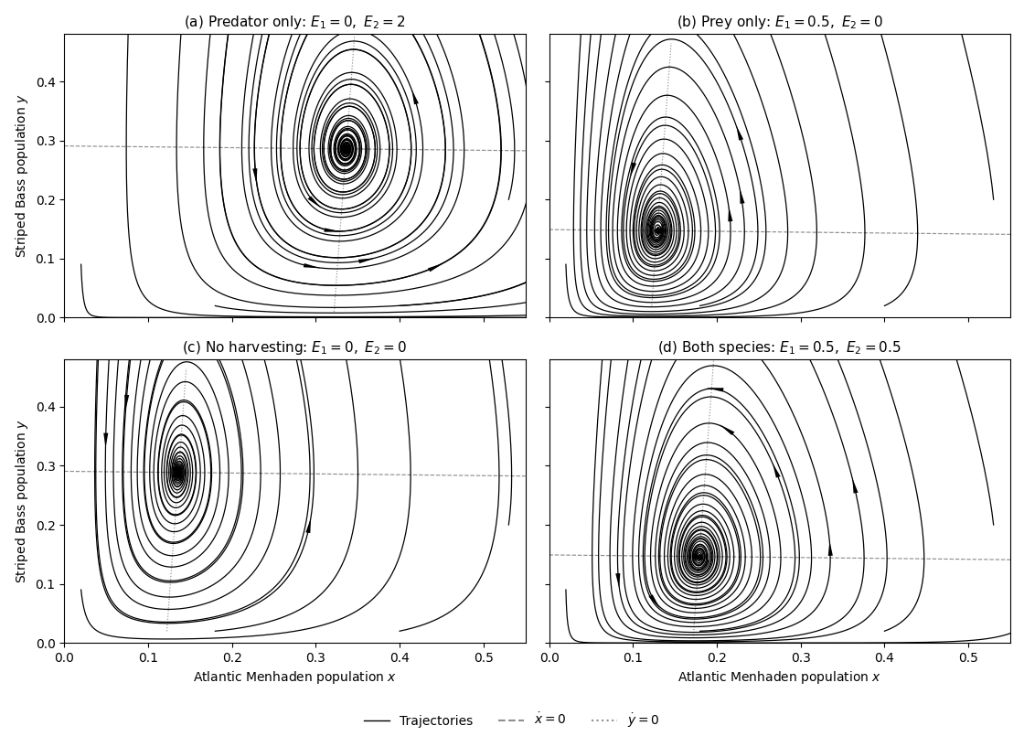
\includegraphics[width=\textwidth]{images/phase_potrait.png}
    \caption{Chân dung pha của hệ trong bốn trường hợp:
    (a) chỉ khai thác Striped Bass;
    (b) chỉ khai thác Atlantic Menhaden;
    (c) không khai thác;
    (d) khai thác đồng thời cả hai loài.}
    \label{fig:phase_portraits}
\end{figure}

Hình~\ref{fig:return_time} thể hiện sự phụ thuộc
của thời gian hồi phục $\tau$ vào cường độ khai thác.
Khi chỉ khai thác Striped Bass, thời gian hồi phục
ban đầu giảm rồi tăng mạnh gần ngưỡng tới hạn.
Ngược lại, khi khai thác Atlantic Menhaden hoặc
đồng thời cả hai loài, thời gian hồi phục tăng
theo cường độ khai thác.

\begin{figure}[htbp]
    \centering
    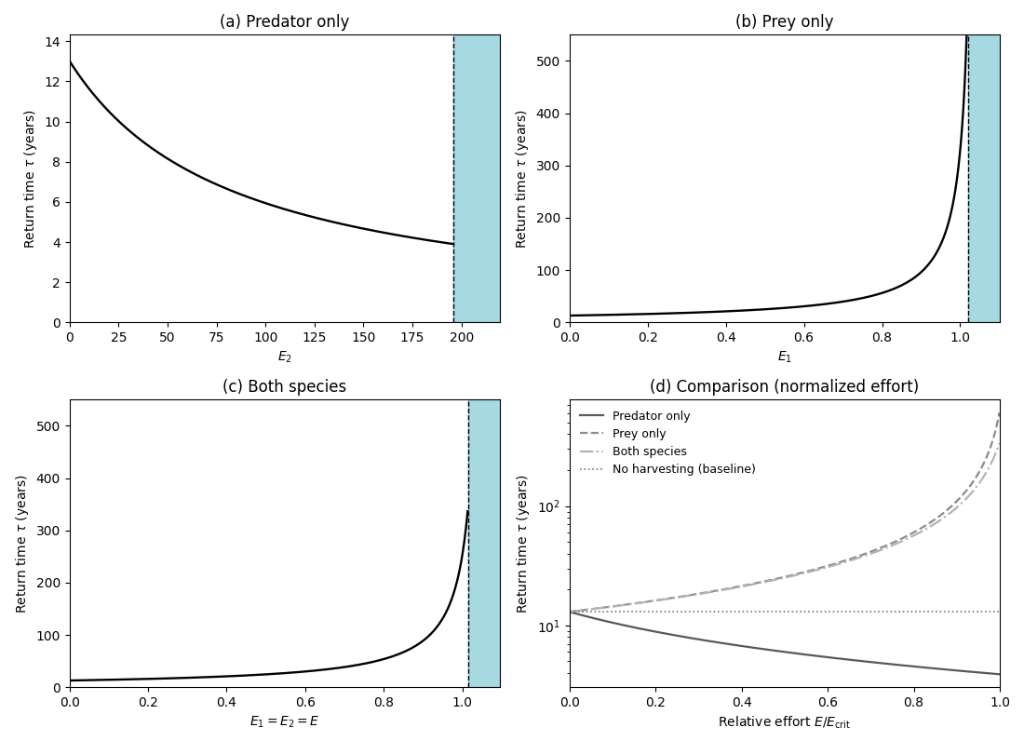
\includegraphics[width=\textwidth]{images/return_time.png}
    \caption{Sự phụ thuộc của thời gian hồi phục $\tau$
    vào cường độ khai thác:
    (a) chỉ khai thác Striped Bass;
    (b) chỉ khai thác Atlantic Menhaden;
    (c) khai thác đồng thời cả hai loài;
    (d) so sánh thời gian hồi phục theo cường độ
    khai thác được chuẩn hóa.}
    \label{fig:return_time}
\end{figure}

